\chapter{Analisi del contesto aziendale}
	\section{L'azienda e il suo ambito di attività}
		PastBook è una piccola azienda con sede ad Amsterdam, nei Paesi Bassi. Essa offre agli utenti la possibilità di creare e stampare
		degli album fotografici personalizzati.
		\begin{figure}[H]
			\centering
			
\includegraphics[width=0.4\textwidth]{capitolo_1/immagini/logo_pastbook.png}
		\end{figure}
		Il progetto nasce nel 2012 quando Stefano Cutello — fondatore e attuale titolare di PastBook — decide di abbandonare il posto di
		lavoro presso eBay per realizzare la propria idea. L'esigenza è quella di riscoprire i ricordi pubblicati ogni giorno sui social
		network: infatti, le vite delle persone sono ormai completamente online e non esiste più niente di stampato.\\
		L'azienda descrive il servizio che essa offre nel seguente modo:
		\hyphenblockquote{english}{Many things can disappear — not your memories. We believe that certain moments can last forever. We
			believe that the best things in the world are not things. We help you rediscover your memories. We collect the highlights of
			your life moments and provide you with a tangible way to relive them — in PastBook.}
		PastBook, dunque, aiuta le persone a raccogliere le proprie foto sparse per il Web e permette loro di creare un album fotografico
		che memorizzi in modo permanente i ricordi più belli.
	\section{Prodotti offerti}
		\subsection{Photo Books in un click}
			Esistono varie aziende che permettono agli utenti di creare album fotografici a partire dalle immagini presenti nei social
			network. PastBook differisce da esse per un importante principio che sta alla base della realizzazione del prodotto: l'utente
			deve poter creare il proprio Photo Book in modo veloce ed automatico, senza pensare a particolari che distolgano la sua mente
			dallo scopo.\\
			L'azienda prevede che i propri clienti debbano solo scegliere il servizio dal quale intendono ottenere le immagini. Il resto
			è automatico: non è previsto che l'utente abbia la possibilità di personalizzare il proprio Photo Book durante la sua
			realizzazione. I più esigenti possono fare piccole modifiche solo a creazione avvenuta.\\
			\begin{multicols}{3}[\noindent PastBook permette di recuperare le immagini utilizzando uno dei seguenti servizi Web:]
				\begin{itemize}
					\item Instagram
					\item Facebook
					\item Flickr
					\item Google Drive
					\item Dropbox
					\item OneDrive
					\item Picasa
					\item Evernote
					\item Box
				\end{itemize}
			\end{multicols}
			\begin{figure}
				\centering
				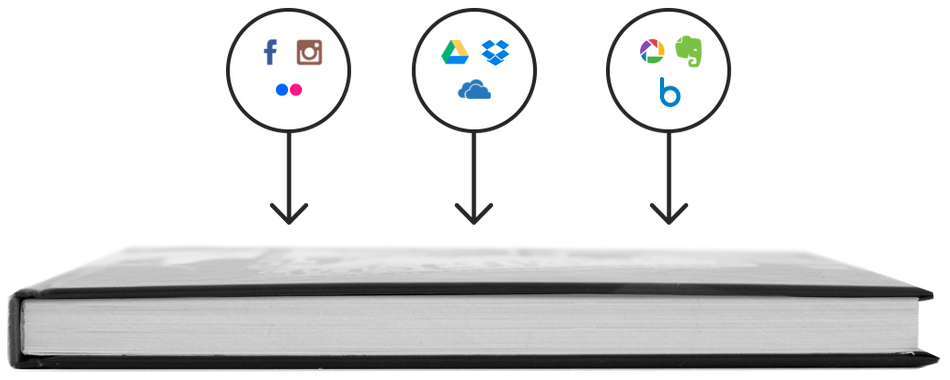
\includegraphics[width=0.9\textwidth]{capitolo_1/immagini/photo_book_one_click.png}
			\end{figure}
			Gli utenti hanno inoltre la possibilità di invitare chiunque ad aggiungere ulteriori ricordi al proprio Photo Book,
			condividendo un link privato tramite email, QR code, Facebook o Twitter.
		\subsection{Photo Books personalizzati}
			PastBook offre anche una seconda tipologia di prodotti: Photo Book creati su misura da designer professionisti. Tale offerta
			è rivolta ai clienti che non pretendono risultati immediati ma che allo stesso tempo esigono una qualità superiore.\\
			Gli utenti, in particolare, dopo aver mandato le proprie foto, possono interagire direttamente con la persona che si sta
			occupando della creazionde del Photo Book per indicare le immagini preferite o per esprimere eventuali preferenze
			riguardanti lo stile, i testi, i colori, etc.
			\begin{figure}[H]
				\centering
				
\includegraphics[width=0.9\textwidth]{capitolo_1/immagini/photo_book_personalizzato.png}
			\end{figure}
	\section{Organizzazione aziendale}
		\subsection{Obiettivi e risultati attesi}
			PastBook persegue obiettivi di tre tipologie differenti:
			\begin{itemize}
				\item tecnici, legati al funzionamento dei prodotti;
				\item economici, legati alla produttività, all'efficacia e all'efficienza;
				\item sociali, legati alla qualità della vita e in particolare alla qualità della vita di lavoro.
			\end{itemize}
			\subsubsection{Qualità del prodotto e dei processi}
				Il principale obiettivo di PastBook è quello di realizzare un algoritmo che sia in grado di produrre in modo
				automatico un Photo Book che sia conforme alle aspettative dei clienti. Oltre a ciò, l'azienda intende raggiungere
				precisi traguardi riguardanti l'efficienza del processo di creazione del prodotto: esso deve avvenire nel minor tempo
				possibile e impiegando una quantità minima di risorse.\\
				Questi obiettivi puramente tecnici celano lo scopo economico di riuscire a vendere i Photo Book realizzati in modo
				automatico ad un prezzo inferiore rispetto a quello proposto della concorrenza, pur mantenendo elevata la
				soddisfazione dei clienti.
			\subsubsection{Semplicità di utilizzo degli strumenti}
				PastBook supporta da sempre una precisa filosofia: gli strumenti a disposizione degli utenti devono essere semplici,
				per non dire basilari. In particolare, l'azienda vuole che il cliente riesca ad ottenere qualcosa di gradito — non
				per forza perfetto — senza sentire il bisogno di dover intervenire per apportare modifiche.\\
				L'uso di questo tipo di approccio si basa sulle seguenti considerazioni:
				\begin{itemize}
					\item Spesso gli utenti provano un nuovo servizio per pura curiosità e, di conseguenza, non sono disposti ad
					utilizzare molto del proprio tempo per giungere al risultato. Numerose possibilità di modifiche e
					personalizzazioni non farebbero altro che spazientire l'utente. Un'azienda deve dunque saper sfruttare il
					breve contatto con il potenziale cliente per poterlo conquistare
					\item Quanto più è il tempo a disposizione di un utente per valutare un acquisto in modo razionale tanto
					meno influiscono su di esso impulsi ed emozioni. È dunque necessario saper cogliere l'irrazionalità iniziale
					del cliente per persuaderlo: per ottenere ciò, la quantità di azioni svolta per creare un Photo Book deve
					essere minima.
				\end{itemize}
			\subsubsection{Valorizzazione del capitale umano}
				Il titolare di PastBook è fermamente convinto che una forte cultura organizzativa sia un fattore critico per le
				performance e il successo dell'azienda. Egli, in particolare, cerca continuamente di motivare e coinvolgere i propri
				dipendenti per fare in modo che essi apprezzino i risultati che il loro lavoro può portare.\\
				In aggiunta, PastBook crede fortemente al fatto che la produttività del personale sia influenzata dalla qualità dei
				rapporti che si instaurano tra le persone facenti parte del team: ciascuno, con le proprie motivazioni, influenza
				positivamente gli altri individui del gruppo, facilitando il raggiungimento dei risultati imposti.\\
				\begin{figure}[H]
	\centering
	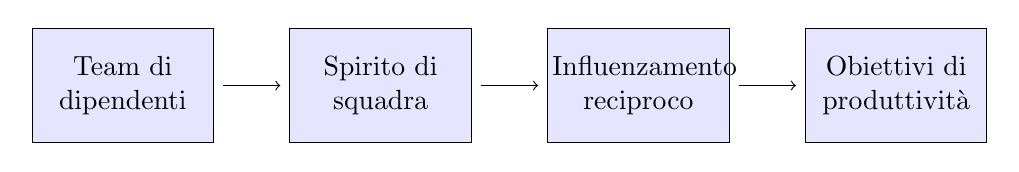
\begin{tikzpicture}
		\draw[fill=blue,fill opacity=0.1] (0,0) rectangle ++(0.19\textwidth,0.12\textwidth);
		\draw (0,0) rectangle ++(0.19\textwidth,0.12\textwidth)
		node[pos=.5, text width=0.18\textwidth, align=center] {Team di dipendenti};
		\draw[->] (0.20\textwidth,0.06\textwidth) -- (0.26\textwidth,0.06\textwidth);
		\draw[fill=blue,fill opacity=0.1] (0.27\textwidth,0) rectangle ++(0.19\textwidth,0.12\textwidth);
		\draw (0.27\textwidth,0) rectangle ++(0.19\textwidth,0.12\textwidth)
		node[pos=.5, text width=0.18\textwidth, align=center] {Spirito di squadra};
		\draw[->] (0.47\textwidth,0.06\textwidth) -- (0.53\textwidth,0.06\textwidth);
		\draw[fill=blue,fill opacity=0.1] (0.54\textwidth,0) rectangle ++(0.19\textwidth,0.12\textwidth);
		\draw (0.54\textwidth,0) rectangle ++(0.19\textwidth,0.12\textwidth)
		node[pos=.5, text width=0.18\textwidth, align=center] {Influenzamento reciproco};
		\draw[->] (0.74\textwidth,0.06\textwidth) -- (0.80\textwidth,0.06\textwidth);
		\draw[fill=blue,fill opacity=0.1] (0.81\textwidth,0) rectangle ++(0.19\textwidth,0.12\textwidth);
		\draw (0.54\textwidth,0) (0.81\textwidth,0) rectangle ++(0.19\textwidth,0.12\textwidth)
		node[pos=.5, text width=0.18\textwidth, align=center] {Obiettivi di produttività};
	\end{tikzpicture}
\end{figure}

				Infine, per fare in modo che ognuno esprima al meglio le proprie potenzialità, l'azienda intende decentralizzare le
				responsabilità ed aumentare l'autonomia decisionale. Parallelamente, ogni dipendente deve cercare di comprendere
				pienamente i limiti entro i quali può operare in modo autonomo.
		\subsection{Risorse disponibili}
			PastBook può avvalersi di numerose risorse per poter raggiungere gli obiettivi prefissati.\\
			Innanzitutto, l'azienda ha a disposizione i propri dipendenti e collaboratori: mentre alcuni di essi forniscono il proprio
			contributo solo per breve tempo, altri lavorano per PastBook in modo stabile. In particolare, durante il periodo in cui ho
			svolto lo stage, l'azienda era composta da 7-9 persone. In aggiunta, alcuni mentori che hanno contribuito a far crescere
			PastBook durante i suoi esordi offrono spesso il proprio aiuto per individuare le strategie vincenti.\\
			Per quanto riguarda le risorse economiche, l'azienda può fare affidamento su una serie di investitori privati che credono
			fortemente nel progetto e nelle persone che lo stanno realizzando. Essi forniscono perlopiù sostegno finanziario e non hanno
			ruoli di tipo decisionale.\\
			Le risorse tecnologiche necessarie all'azienda sono molto poche. Infatti, ogni persona lavora utilizzando il proprio PC e
			solo in casi particolari utilizza dispositivi di altro tipo.\\
			Per quanto riguarda gli spazi, infine, i dipendenti di PastBook possono usufruire, oltre che dell'ufficio, anche di due
			cucine e di una sala relax.
		\subsection{Componenti e relazioni organizzative}
			\subsubsection{Funzioni e ruoli}
				In PastBook le responsabilità di ciascuna persona sono ben definite. Questo aiuta i dipendenti a capire i propri
				confini operativi e a diminuire le dimenticanze.\\
				L'azienda — per funzionare in modo corretto — necessita dei seguenti ruoli:
				\begin{center}
					\rowcolors{1}{azzurro_chiaro}{azzurro}
					\begin{tabular}[H]{p{0.25\textwidth} p{0.60\textwidth}}
						Dirigente 			& Si occupa della gestione delle risorse disponibili e del
										  coordinamento generale per poter raggiungere gli obiettivi
										  prefissati.\\
						\hline
						Responsabile finanziario	& Si occupa della gestione e della supervisione delle attività
										  finanziarie.\\
						\hline
						Responsabile del marketing	& Si occupa della comunicazione sui social media, attuando strategie
										  per aumentare il valore percepito dai consumatori rispetto al
										  prodotto offerto.\\
						\hline
						Customer relationship manager	& Si occupa della gestione delle relazioni con i clienti. Questo
										  implica un approccio operativo (risposte tempestive ed efficaci
										  alle richieste) e uno analitico (analisi dei bisogni e della
										  soddisfazione per sviluppare un'offerta commerciale appropriata).\\
						\hline
						Grafico				& Fornisce supporto e consulenza artistica durante la progettazione
										  dei vari prodotti (sito web, applicazioni mobile, banner
										  pubblicitari, etc.).\\
						\hline
						Chief technical officer		& Supervisiona l'implementazione dei prodotti e dei servizi offerti
										  per assicurare che portino valore aggiunto all'azienda. Coglie le
										  potenzialità di nuove tecnologie per convertirle in decisioni
										  strategiche per l'azienda.\\
						\hline
						Sviluppatore 			& Si occupa dei vari aspetti del ciclo di vita di un prodotto
										  software.\\
					\end{tabular}
				\end{center}
				Alcuni dipendenti aziendali, a seconda delle necessità, possono ricoprire più di una mansione.
			\subsubsection{Struttura organizzativa}
				L'azienda è suddivisa in tre unità organizzative, individuate sulla base degli obiettivi che ognuna di esse si impone
				di raggiungere:
				\begin{itemize}
					\item all'\emph{area amministrativa}, che si occupa di aspetti economici e decisionali, appartengono il
					dirigente e il responsabile finanziario;
					\item all'\emph{area commerciale}, che si occupa delle strategie di mercato, della commercializzazione del
					prodotto e dell'assistenza ai clienti, appartengono tutti i membri del front office e il responsabile del
					marketing;
					\item all'\emph{area ricerca e sviluppo}, che studia come migliorare i prodotti o come crearne di nuovi,
					appartengono il CTO, gli sviluppatori e il grafico.
				\end{itemize}
				\begin{figure}[H]
	\centering
	\begin{tikzpicture}
		\draw[fill=azzurro] (0,0) rectangle ++(0.20\textwidth,0.12\textwidth);
		\draw (0,0) rectangle ++(0.20\textwidth,0.12\textwidth)
		node[pos=.5, text width=0.18\textwidth, align=center] {Area commerciale};
		\draw[fill=azzurro] (0.56\textwidth,0) rectangle ++(0.20\textwidth,0.12\textwidth);
		\draw (0.56\textwidth,0) rectangle ++(0.20\textwidth,0.12\textwidth)
		node[pos=.5, text width=0.18\textwidth, align=center] {Area ricerca e sviluppo};
		\draw[fill=azzurro] (0.28\textwidth,0.13\textwidth) rectangle ++(0.20\textwidth,0.12\textwidth);
		\draw (0.28\textwidth,0.13\textwidth) rectangle ++(0.20\textwidth,0.12\textwidth)
		node[pos=.5, text width=0.18\textwidth, align=center] {Area amministrativa};
		\draw (0.21\textwidth,0.06\textwidth) -- (0.55\textwidth,0.06\textwidth);
		\draw (0.38\textwidth,0.06\textwidth) -- (0.38\textwidth,0.12\textwidth);
	\end{tikzpicture}
\end{figure}

				PastBook, essendo una realtà aziendale molto piccola, non prevede la presenza di organi di comando e relativi
				subordinati. Tuttavia, per ognuna delle unità organizzative è possibile individuare una persona che funge da
				riferimento per i colleghi: una sorta di leader informale, che trae la sua legittimazione dal consenso degli altri
				membri.\\
				Molto spesso — per far fronte a nuovi problemi o per tentare di raggiungere specifici obiettivi — persone provenienti
				da unità diverse formano dei gruppi di lavoro temporanei, non descrivibili all'interno dell'organigramma. Questi
				gruppi sono formati per sfruttare competenze in ambiti diversi e per affrontare i problemi da diversi punti di vista.
				Accade spesso, per esempio, che gli esperti di marketing collaborino con i membri dell'area ricerca e sviluppo per
				poter realizzare un prodotto di valore sia dal punto di vista funzionale che commerciale.
			\subsubsection{Coordinamento e controllo}
				Descrivo come viene controllata e coordinata l'azienda. In particolare descrivo come l'azienda usi il metodo scrum,
				con standup giornalieri nei quali ognuno spiega cosa ha fatto, cosa intende fare, se ha particolari problemi o se è
				disponibile ad aiutare un collega. Descrivo inoltre le più corpose riunioni mensili nei quali ognuno è invitato a
				portare la propria idea in relazione ai vari problemi che l'azienda si ritrova ad affrontare. Descrivo inoltre quale
				tecnologia viene utilizzata per fare in modo si sappia sempre ognuno cosa sta facendo (sempre seguendo lo scrum).
			\subsubsection{Gestione del personale}
				\paragraph{Selezione, valutazione e formazione}
					Descrivo il fatto che per l'azienda risulti molto importante il fatto che una persona sia indipendente nel
					lavorare e soprattutto nel valutare un problema e nel prendere personalmente una decisione sensata.
					Descrivo inoltre come l'azienda attui percorsi di affiancamento e formativi per la persona che entra a far
					parte del gruppo (consentono di capire sia il modo di lavorare ma anche credenze, valori, regole che di
					solito non sono formalizzate).
				\paragraph{Motivazione e coinvolgimento}
					Il lavoro all'interno di PastBook non consiste in un semplice scambio \emph{energia-fatica-ricompensa}: esso
				rappresenta piuttosto un mezzo per la crescita personale e un'opportunità di espressione delle persone nell'ambiente
				che le circonda.\\
					Descrivo come l'azienda cerchi in modo costante di fare in modo che ognuno si senta coinvolto nel progetto
					(soprattutto intraprendendo spesso confronti su problemi delle tipologie più disparate per fare in modo che
					ognuno possa presentare la propria idea e/o soluzione).
					Descrivo come si cerchi continuamente di fare in modo che si creino legami anche di amicizia fra colleghi,
					proponendo spesso attività terze da svolgere tutti insieme, eventualmente anche durante l'orario di lavoro.
			\subsubsection{Gestione dei clienti}
				Descrivo come vengono gestiti i clienti in azienda. In particolare mi soffermo sul fatto che la gestione dei vecchi
				e dei potenziali clienti avviene su due fronti: assistenza personalizzata per problemi durante la creazione dei libri
				e mantenimento di un blog nel quale vengono inseriti sia suggerimenti su come usare gli strumenti messi a
				disposizione dall'azienda sia fatti, eventi e curiosità che possono stuzzicare la mente del lettore. L'azienda
				prevede del personale dedicato esclusivamente a ciascuna di queste due aree.
			\subsubsection{Comunicazione nell'azienda}
				Qui descrivo sia il modo in cui si comunica in azienda (prevalentemente contatti informali, fortemente basati sulle
				relazioni, senza la presenza di una struttura gerarchica o di un forte grado di controllo) sia gli strumenti e/o le
				tecnologie utilizzati per fare ciò.
	\section{Sviluppo software}
		\subsection{Metodologia di lavoro}
			\subsubsection{Tipico ciclo di vita del software}
				Descrizione generale di come nell'azienda un'idea nasca, cresca e venga infine sviluppata. In particolare sottolineo
				come un'idea derivi solitamente da uno dei meeting mensili fatti tutti insieme. Proseguo dicendo come l'idea viene
				sviluppata e come si crei eventualmente un piccolo gruppo che prosegue nella definizione e nello sviluppo dei
				concetti elaborati dall'intero team. Dico infine che in base alla tipologia di prodotto questo venga testato solo
				internamente o anche con l'aiuto di beta tester esterni all'azienda.
			\subsubsection{Analisi dei requisiti}
				Descrivo come si svolge l'analisi dei requisiti. Essa è molto informale ed è aperta non solo agli sviluppatori, ma
				anche ad altri ruoli aziendali. Descrivo inoltre come l'informale "documentazione" (immagini, diagrammi, appunti)
				viene prodotta e poi memorizzata.
			\subsubsection{Progettazione e codifica}
				Descrivo la progettazione e la codifica, che in azienda arrivano quasi a coincidere (non esiste un momento in cui
				si pensi solo alla progettazione e di conseguenza non esiste nemmeno una documentazione di qualsiasi tipo che la
				riguardi, con tutti i problemi del caso). Descrivo come gli sviluppatori collaborino durante tali attività.
			\subsubsection{Beta testing}
				Alcuni prodotti e/o strumenti realizzati vengono distribuiti dall'azienda a delle persone incaricate di testarli
				e di rilasciare dei feedback, in modo tale che si possano apportare dei miglioramenti. Questa è l'unica forma di
				test che viene fatta in modo sistematico. Descrivo in questa sezione chi ha accesso ai prodotti in anteprima, quali
				sono gli strumenti che lo permettono e come si analizzano i dati provenienti dai feedback.
		\subsection{Tecnologie, tecniche e strumenti utilizzati}
			\subsubsection{Generazione di un Photo Book}
				Descrivo in modo molto generale come l'azienda produce il pdf che rappresenta il libro fotografico che poi viene
				successivamente stampato. Descrivo inoltre le tecnologie che sono utilizzate durante questo processo.
			\subsubsection{API e services}
				Comincio con il descrivere brevemente il server dell'azienda (tecnologie utilizzate e architettura generale). In
				seguito mi concentro su due componenti fondamentali di tale architettura che sono a disposizione degli sviluppatori:
				API REST (richieste basilari per creare/modificare un album fotografico) e services (richieste complesse e
				strutturate per l'esecuzione automatica di alcuni compiti).
			\subsubsection{Ambiente di lavoro virtuale}
				Descrivo come gli sviluppatori utilizzino un ambiente di lavoro virtuale che simuli in tutto e per tutto quello
				reale, in modo tale da non dover lavorare direttamente sui prodotti accessibili al pubblico. Descrivo le tecnologie
				utilizzate per la creazione di tale ambiente.
	\section{Propensione all'innovazione}
		Descrivo il rapporto che l'azienda ha con l'innovazione, in relazione anche alla tipologia di utenti alla quale si rivolge.
